\documentclass{article}
\usepackage{graphicx}
\usepackage{amsmath}
\usepackage{esvect}
\usepackage{setspace}
\usepackage{hyperref}
\usepackage{amsfonts}

\DeclareMathOperator{\sech}{sech}
\DeclareMathOperator{\csch}{csch}
\DeclareMathOperator{\arcsec}{arcsec}
\DeclareMathOperator{\arccot}{arccot}
\DeclareMathOperator{\arccsc}{arccsc}
\DeclareMathOperator{\arccosh}{arccosh}
\DeclareMathOperator{\arcsinh}{arcsinh}
\DeclareMathOperator{\arctanh}{arctanh}
\DeclareMathOperator{\arcsech}{arcsech}
\DeclareMathOperator{\arccsch}{arccsch}
\DeclareMathOperator{\arccoth}{arccoth}

\newcommand{\mysubsection}[1]{
    \subsubsection*{#1}
    \addcontentsline{toc}{subsection}{#1}
    \vspace{-1em}
    \rule{\linewidth}{.1mm}
    \par
}


\begin{document}

    \pagenumbering{roman}
    \tableofcontents

    \pagebreak

    \pagenumbering{arabic}

    \begin{center}
        \subsection*{Vectors and the Geometry of Space}
        \addcontentsline{toc}{section}{Vectors and the Geometry of Space}
    \end{center}

    \medskip
    \mysubsection{The Dot Product}

    \smallskip\noindent
    The dot product, or scalar product, of vectors $u$ and $v$:
    \begin{gather*}
        u\cdot v=\left|u\right|\left|v\right|\cos\theta
        \qquad
        \theta=\arccos\frac{u\cdot v}{\left|u\right|\left|v\right|} \\
        u\cdot v = u_1 v_1+u_2 v_2+u_3 v_3
    \end{gather*}

    \smallskip\noindent
    For two non-zero vectors $u$ and $v$;
    \begin{align*}
        \quad &u\cdot v >0 \quad \Longleftrightarrow \quad \theta<90^{\circ} \\
        \quad &u\cdot v =0 \quad \Longleftrightarrow \quad \theta=90^{\circ} \\
        \quad &u\cdot v <0 \quad \Longleftrightarrow \quad \theta>90^{\circ}
    \end{align*}

    \smallskip\noindent
    The vector projection of $u$ onto $v$ is equal to the scalar component of $u$ in the direction of $v$ times the direction of $v$.
    Using the definition of the dot product, this can be rearranged into a form more easily evaluated by hand.
    \[
        \text{proj}_v u = \left(\left|u\right|\cos\theta\right)\frac{v}{\left|v\right|}
        =
        \frac{u\cdot v}{\left|v\right|^2}\,v
    \]

    \smallskip
    \mysubsection{The Cross Product}

    \smallskip\noindent
    The cross product $u\times v$ where $n$ is a unit vector normal to the plane formed by $u$ and $v$.
    Because $n$ is a unit vector, the magnitude of $u \times v$ is readily apparent. $\left|u\times v\right|$ is the area of the parallelogram formed by the vectors.
    \begin{gather*}
        u\times v = \left(\left|u\right|\left|v\right|\sin\theta\right)n    \\[.3em]
        \left|u\times v\right| = \left|u\right|\left|v\right|\sin\theta
    \end{gather*}

    \medskip\noindent
    Two non-zero vectors $u$ and $v$ are parallel if and only if $u\times v = 0$
    \[
        u \left|\right| v \quad \Longleftrightarrow \quad u\times v = 0
    \]

    \medskip\noindent
    Calculating the cross product as a determinant:
    \[
        u\times v =
        \begin{vmatrix}
            i   & j   & k   \\
            u_1 & u_2 & u_3 \\
            v_1 & v_2 & v_3
        \end{vmatrix} =
        \begin{aligned}
            &i\left(u_2 v_3-u_3 v_2\right)- \\
            &j\left(u_1 v_3-u_3 v_1\right)+ \\
            &k\left(u_1 v_2-u_2 v_1\right)
        \end{aligned}
    \]

    \medskip\noindent
    The triple scalar product, or box product, is the volume of the parallelepiped formed by vectors $u$, $v$ and $w$.
    It can be calculated as a determinant:
    \[
        \left(u\times v\right)\cdot w =
        \begin{vmatrix}
            u_1 & u_2 & u_3 \\
            v_1 & v_2 & v_3 \\
            w_1 & w_2 & w_3
        \end{vmatrix}
    \]

    \smallskip
    \mysubsection{Equations of Lines and Planes in Space}

    \smallskip\noindent
    The standard parameterization of the line through $P\left(x_0,y_0,z_0\right)$ parallel to a nonzero vector $v = \langle v_1,v_2,v_3\rangle$
    \[
        x=x_0+tv_1,\quad y=y_0+tv_2,\quad z=z_0+tv_3
    \]

    \smallskip\noindent
    The distance from a point $S$ to a line that passes through point $P$ parallel to vector $v$ is

    \begin{samepage}
        \begin{minipage}[t]{0.4\textwidth}
            \begin{align*}
                d &= |\vv{PS}|\sin\theta \\\\
                d &= \frac{|\vv{PS}\times v|}{|v|}
            \end{align*}
        \end{minipage}
        \begin{minipage}[t]{0.4\textwidth}
            \centering
            \raisebox{-1.1in}{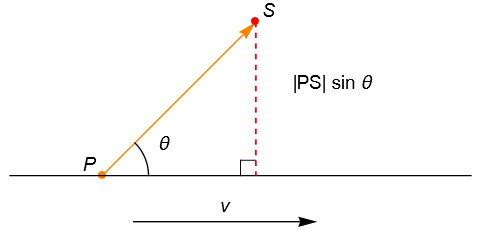
\includegraphics[scale=0.5]{distancePointToLine}}
        \end{minipage}
    \end{samepage}

    \vspace{1.5em}
    \smallskip\noindent
    A plane can be defined by its normal vector $n$.
    The plane containing point $P_0$ consists of all points where $n$ and $\vv{P_0 P}$ are perpendicular, where $P$ is any point.
    The equation of a plane through $P_0\left(x_0,y_0,z_0\right)$ normal to a nonzero vector $n=\langle a, b, c \rangle$ can be expressed as

    \vspace{-1em}
    \begin{minipage}[t]{0.5\textwidth}
        \begin{align*}
            &n\cdot \vv{P_0 P} = 0                                          \\[.3em]
            &a\left(x-x_0\right)+b\left(y-y_0\right)+c\left(z-z_0\right)=0  \\[.3em]
            &ax+by+cz=d \text{,}                                            \\
            &\quad\text{where } d=ax_0+by_0+cz_0
        \end{align*}
    \end{minipage}
    \begin{minipage}[t]{0.4\textwidth}
        \centering
        \raisebox{-1.2in}{\includegraphics[scale=0.7]{placeholder}}
    \end{minipage}

    \smallskip\noindent
    If $P$ is a point on a plane with normal vector $n$, then the distance from any point $S$ to the plane is the length of the vector projection of $\vv{PS}$ onto $n$:
    \[
        d=\left|\vv{PS}\cdot\frac{n}{|n|}\right|
    \]

    \smallskip\noindent
    The angle between two intersecting planes is defined to be the acute angle between their normal vectors.
    \[
        \theta=\arccos{\frac{n_1\cdot n_2}{|n_1||n_2|}}
    \]

    \pagebreak
    \begin{center}
        \subsection*{Vector-Valued Functions and Space Curves}
        \addcontentsline{toc}{section}{Vector-Valued Functions and Space Curves}
    \end{center}

    \medskip
    \mysubsection{Curves in Space and Their Tangents}

    \smallskip\noindent
    The vector function $r\left(r\right) = f\left(t\right)i+g\left(t\right)j+h\left(t\right)k$ has a derivative at $t$ if $f$, $g$ and $h$ have derivatives at $t$.
    \[
        r'\left(t\right) = \frac{dr}{dt} = \frac{df}{dt}i+\frac{dg}{dt}j+\frac{dh}{dt}k
    \]

    \smallskip\noindent
    Let $u$ and $v$ be differentiable vector functions of $t$, and $f$ be any differentiable scalar function.
    \begin{align*}
        &\text{Dot Product:} &&\frac{d}{dt}\left[u(t)\cdot v(t)\right] = u'(t)\cdot v(t)+u(t)\cdot v'(t) \\
        &\text{Cross Product:} &&\frac{d}{dt}\left[u(t)\times v(t)\right] = u'(t)\times v(t)+u(t)\times v'(t)\\
        &\text{Chain Rule:} &&\frac{d}{dt}\left[u\left(f(t)\right)\right] = f'(t)\,\,u'\left(f(t)\right)
    \end{align*}

    \smallskip
    \mysubsection{Arc Length and Curvature}

    \smallskip\noindent
    The length of a smooth curve $r(t) = \langle \, x(t), y(t), z(t) \, \rangle$ , $a \leq t \leq b$ from $t=a$ to $t=b$ is
    \begin{align*}
        L &= \int_a^b \sqrt{\left(\frac{dx}{dt}\right)^2 + \left(\frac{dy}{dt}\right)^2 + \left(\frac{dz}{dt}\right)^2}\,dt = \int_a^b \left| v \right| \,dt
    \end{align*}

    \smallskip\noindent
    Arc length parameterization with starting point $P_{t_0}$
    \[
        s(t)=\int_{t_0}^t\left| v\left(\tau\right) \right| \, d\tau
    \]

    \smallskip\noindent
    The velocity vector $v=dr/dt$ is tangent to the curve $r(t)$, therefore
    \[
        T=\frac{v}{|v|}
    \]
    \noindent
    is a unit vector tangent to the (smooth) curve, called the \emph{unit tangent vector}.

    \medskip\noindent
    If $T$ is the unit vector of a smooth curve, then the curvature function of the curve is
    \[
        \kappa=\left| \frac{dT}{ds} \right|
        = \left| \frac{dT}{dt}\,\frac{dt}{ds} \right|
        = \frac{1}{|ds/dt|}\left|\frac{dT}{ds} \right|
        = \frac{1}{|v|}\left|\frac{dT}{dt}\right|
    \]

    \smallskip\noindent
    At a point where $\kappa \neq 0$, the principal unit normal vector for a smooth curve in the plane is
    \[
        N=\frac{1}{\kappa}\frac{dT}{ds} = \frac{dT/dt}{\left|dT/dt\right|}
    \]

    \smallskip\noindent
    The principal normal vector will point to the concave side of the curve.

    \pagebreak

    \begin{center}
        \subsection*{Partial Derivatives}
        \addcontentsline{toc}{section}{Partial Derivatives}
    \end{center}

    \medskip
    \mysubsection{Functions of Several Variables}

    \smallskip\noindent
    Level curves for a given $z$ are found my setting $z=f(x,y)$ to be a constant, then finding the resulting curve in the $x,y$ plane.

    \smallskip
    \mysubsection{Limits of Functions of Several Variables}

    \medskip\noindent
    \[
        \lim_{(x_1 , \dots , x_n)\rightarrow(a_1 , \dots , a_n)} f(x_1 , \dots , x_n) = L
    \]
    means that, given an $\epsilon>0$ we can find a $\delta>0$ such that
    \[
        \left|f(x_1 , \dots , x_n)-L\right|<\epsilon \text{\quad whenever\quad} 0<\sqrt{(x_1 - a_1 )^2 + \dots + (x_n - a_n)^2}<\delta
    \]

    \medskip\noindent
    Interestingly, any polynomial is continuous on $\mathbb{R}^2$, and any rational function is continuous on its domain.
    We can verify this by looking at the properties of limits; the limit of a sum is the sum of the limits, the limit of a product is the product of the limits, etc.

    \smallskip
    \mysubsection{Partial Derivatives}

    \smallskip\noindent
    A partial derivative is the derivative of a function with respect to one variable while the other variables are fixed.
    \begin{gather*}
        \frac{\partial}{\partial x_i}f(x_1,\dots,x_i,\dots x_n) = \lim_{h\rightarrow 0}\frac{f(x_1,\dots,x_i+h,\dots x_n)-f(x_1,\dots,x_i,\dots x_n)}{h}
    \end{gather*}

    \medskip\noindent
    The partial derivative can be notated in different ways:
    \begin{gather*}
        \frac{\partial}{\partial x}f(x,y) = \frac{\partial f}{\partial x} = f_x(x,y)=f_x=D_x f                                           \\[.4em]
        \frac{\partial^2}{\partial^2 x}f(x,y) = \frac{\partial f}{\partial^2 x} = f_{xx}(x,y)=f_{xx}=D_{xx}f                            \\[.4em]
        \frac{\partial^2}{\partial x \, \partial y}f(x,y) = \frac{\partial f}{\partial x \, \partial y} = f_{xy}(x,y)=f_{xy}=D_{xy}f
    \end{gather*}

    \smallskip\noindent
    It is important to note that $\partial f /\partial x$ \emph{cannot} be interpreted as a ratio of differentials as it would with the total derivative $df/dx$

    \medskip\noindent
    Clairaut's Theorem, or, symmetry of second derivatives: If the second partial derivatives of a function are continuous, the order of differentiation does not matter.
    This can also be extended to higher order partial derivatives if their functions are continuous.

\end{document}
